%
%
%آیین‌نامه حق مالکیت مادی و معنوی
%
%
%در این فایل، کافی است در ابتدا، عبارت‌های موجود در خط‌های 33، 37، 41، 45، 57 و 60 را پاک و بعد، اطلاعات خود را تایپ کنید. 
%در خط 57، برای وارد کردن تصویر امضای خود به شکل عکس و با فرمت jpg، در ابتدا فایل Signature.jpg را در پوشه Figures حذف و تصویر امضای خود را با همان نام در همان پوشه اضافه کنید. (در صورتی که فرمت عکس jpg نباشد، در خط 57، عبارت jpg را از Signature.jpg حذف و فرمت جدید را اضافه کنید)
%
%
\begin{center}
\textbf{
آیین‌نامه حق مالکیت مادی و معنوی در مورد نتایج پژوهش‌های علمی دانشگاه تربیت مدرس
}
\end{center}
\thispagestyle{empty}
%دستور زیر برای تغییر اندازه کل متنی است که بعد از این دستور می‌آید.
\fontsize{3.4mm}{3.4mm}\selectfont \textbf{
مقدمه:
}
با عنایت به سیاست‌های پژوهشی و فناوری دانشگاه در راستای تحقق عدالت و کرامت انسان‌ها که لازمه شکوفایی علمی و فنی است و رعایت حقوق مادی و معنوی دانشگاه و پژوهشگران، لازم است اعضای هیأت علمی، دانشجویان، دانش‌آموختگان و دیگر همکاران طرح، در مورد نتایج پژوهش‌های علمی که تحت عناوین پایان‌نامه، رساله و طرح‌های تحقیقاتی با هماهنگی دانشگاه انجام شده است، موارد زیر را رعایت نمایند:

ماده 1- حق نشر و تکثیر پایان‌نامه/رساله و درآمدهای حاصل از آنها متعلق به دانشگاه می‌باشد ولی حقوق معنوی پدیدآورندگان محفوظ خواهد بود.

ماده 2- انتشار مقاله یا مقالات مستخرج از پایان‌نامه/رساله به صورت چاپ در نشریات علمی و یا ارائه در مجامع علمی باید به نام دانشگاه بوده و با تأیید استاد راهنمای اصلی، یکی از اساتید راهنما، مشاور و یا دانشجو مسئول مکاتبات مقاله باشد. ولی مسئولیت علمی مقاله مستخرج از پایان‌نامه/رساله به عهده اساتید راهنما و دانشجو می‌باشد. 

تبصره: در مقالاتی که پس از دانش‌آموختگی به صورت ترکیبی از اطلاعات جدید و نتایج حاصل از پایان‌نامه/رساله منتشر می‌شود نیز باید نام دانشگاه درج شود.

ماده 3- انتشار کتاب، نرم‌افزار و یا آثار ویژه (اثری هنری مانند فیلم، عکس، نقاشی و نمایش‌نامه) حاصل از نتایج پایان‌نامه/رساله و تمامی طرح‌های تحقیقاتی کلیه واحدهای دانشگاه اعم از دانشکده‌ها، مراکز تحقیقاتی، پژوهشکده‌ها، پارک علم و فناوری و دیگر واحدها باید با مجوز کتبی صادره از معاونت پژوهشی دانشگاه و بر اساس آیین‌نامه‌ها مصوب انجام شود.

ماده 4- ثبت اختراع و تدوین دانش فنی و یا ارائه یافته‌ها در جشنواره‌های ملی، منطقه‌ای و بین‌المللی حاصل نتایج مستخرج از پایان‌نامه/رساله و تمامی طرح‌های تحقیقاتی دانشگاه باید با هماهنگی استاد راهنما یا مجری طرح از طریق معاونت پژوهشی دانشگاه انجام گیرد.

ماده 5- این آیین‌نامه در 5 ماده و یک تبصره در تاریخ 01/04/1387 در شورای پژوهشی و در تاریخ 23/04/1387 در هیأت رئیسه دانشگاه به تأیید رسید و در جلسه مورخ 15/07/1387 شورای دانشگاه به تصویب رسیده و از تاریخ تصویب در شورای دانشگاه لازم‌الاجرا است.

«اینجانب 
\textbf{
نام خود را وارد کنید
}
دانشجوی رشته 
\textbf{
نام رشته خود را وارد کنید
}
ورودی سال تحصیلی 
\textbf{
سال ورود خود را وارد کنید
}
مقطع 
\textbf{
مقطع خود را وارد کنید
}
دانشکده 
\textbf{
علوم ریاضی 
}
متعهد می‌شوم کلیه نکات مندرج در آیین‌نامه حق مالکیت مادی و معنوی در مورد نتایج پژوهش‌های علمی دانشگاه تربیت مدرس را در انتشار یافته‌های علمی مستخرج از پایان‌نامه/رساله تحصیلی خود رعایت نمایم. در صورت تخلف از مفاد آیین‌نامه فوق‌الاشعار به دانشگاه وکالت و نمایندگی می‌دهم که از طرف اینجانب نسبت به لغو امتیاز اختراع به نام بنده و یا هر گونه امتیاز دیگر و تغییر آن به نام دانشگاه اقدام نماید. ضمناً نسبت به جبران فوری ضرر و زیان حاصله بر اساس برآورد دانشگاه اقدام خواهم نمود و بدین وسیله حق هر گونه اعتراض را از خود سلب نمودم.» 
\begin{flushleft}
\makebox[3cm]{
امضا:
}
\\
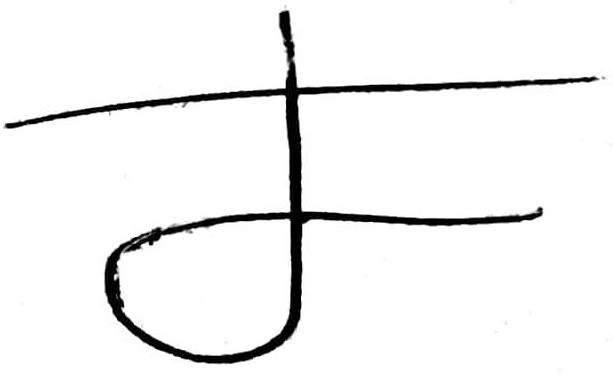
\includegraphics[scale=0.2]{Signature.jpg}
\\
تاریخ:
تاریخ را وارد کنید
\end{flushleft}